\section{Lengua de Señas}
Desde tiempos remotos, las personas con discapacidad auditiva han enfrentado significativos desafíos comunicativos, lo que les llevó a desarrollar su propio sistema de comunicación. Así surgió la lengua de señas, un conjunto estructurado de gestos visuales que permite a la comunidad sorda expresar ideas y emociones. Esta lengua, al igual que otras, está regida por normas lingüísticas establecidas por comunidades sordas \cite{MarzoPena2022}.

\subsection{Historia de la lengua de señas}
La lengua de señas se desarrolló de manera independiente por la comunidad sorda para satisfacer sus necesidades comunicativas. Históricamente estigmatizada y mal entendida, era considerada un lenguaje de gestos simple hasta que investigaciones realizadas en 1960 por William Stokoe revelaron su capacidad para expresar ideas complejas y estructuradas \cite{RodriguezVelasquezSF}.

En el siglo XVIII, el Abad Charles-Michel de L’Epée fundó la primera escuela pública para sordos, marcando un cambio trascendental en la educación de esta comunidad, utilizando la lengua de señas como principal medio de enseñanza. Este avance no solo facilitó la comunicación y el aprendizaje, sino que también permitió que los sordos desempeñaran roles activos como educadores. La metodología de L’Epée se expandió internacionalmente, influyendo en la creación de escuelas y en el desarrollo de nuevas lenguas de señas \cite{RodriguezVelasquezSF}.

Durante los siglos XIX y XX, las lenguas de señas ganaron reconocimiento como sistemas lingüísticos completos y estructurados, capaces de expresar una gama completa de ideas y emociones. En el siglo XX, el reconocimiento de los derechos lingüísticos de las comunidades sordas se amplió significativamente, afirmando la importancia de las lenguas de señas como herramientas educativas y culturales esenciales \cite{RodriguezVelasquezSF}.

A raíz de la necesidad de comunicación en las comunidades sordas, cada país ha desarrollado su propia lengua de señas, integrando a menudo estructuras de lenguas de señas extranjeras, como el \textit{American Sign Language (ASL)}, así como señas locales únicas. Esto ha dado lugar a que cada país, e incluso regiones dentro de los mismos, tengan su propia lengua de señas con estructuras gramaticales y léxicos distintos \cite{RuizVilla2022}.

\subsection{Lengua de Señas en la Actualidad}
En la actualidad, la lengua de señas se está adaptando a un entorno globalizado y tecnológicamente avanzado, donde las necesidades comunicativas evolucionan constantemente. Estos cambios han impulsado la creación de legislaciones, políticas, formación de asociaciones y el desarrollo de nuevas tecnologías destinadas a minimizar las barreras comunicativas. Un ejemplo significativo es la iniciativa de las Naciones Unidas al proclamar el 23 de septiembre como Día Internacional de las Lenguas de Señas, enfatizando la importancia de estas lenguas \cite{Parada2022}.

Sin embargo, a pesar de estos avances, persisten desafíos significativos. La falta de uniformidad de las lenguas de señas a nivel global requiere que las personas aprendan la lengua de señas específica de cada comunidad, lo cual impide la existencia de una forma de comunicación internacional uniforme \cite{RuizVilla2022}.

Además, la lengua de señas, a menudo catalogada como una lengua minoritaria, es aprendida solamente por una pequeña fracción de la población sin discapacidades auditivas. Esta limitada difusión crea una brecha de comunicación significativa, contribuyendo a la marginación de la comunidad sorda y limitando su participación plena en actividades sociales y económicas. Esto subraya la necesidad de una mayor educación y sensibilización sobre la lengua de señas para promover una verdadera inclusión \cite{MelendezLabrador2021}.

\section{Lengua de Señas de Guatemala (LENSEGUA)}
\subsection{Historia}
La Lengua de Señas de Guatemala (LENSEGUA) ha evolucionado como una herramienta vital de comunicación para la comunidad sorda guatemalteca. Aunque su desarrollo específico ha sido menos documentado en comparación con lenguas de señas de otros países, LENSEGUA ha sido influenciada tanto por “Señas Caseras ” de diferentes departamentos del país como por interacciones con lenguas de señas de otros países \cite{Aroche2022} \cite{EndangeredLanguages}.

Antes de la formalización del uso de LENSEGUA, no existía un manual estandarizado que facilitara el aprendizaje de la lengua de señas guatemalteca. Hoy en día de hecho todavía existen diferencias entre las señas utilizadas en los departamentos del país. Sin embargo, en julio de 2001, el Comité Pro Ciegos y Sordos de Guatemala, una institución pionera en la educación y rehabilitación de personas con discapacidad auditiva, publicó el primer manual oficial para el aprendizaje de LENSEGUA. Este manual representó un avance crucial en la estandarización y enseñanza de la lengua de señas, proporcionando un recurso esencial para los estudiantes, profesionales y la comunidad en general interesada en aprender este método de comunicación \cite{deLeon2021}.

\subsection{Legislación}
En términos legislativos, Guatemala ha hecho avances significativos en la última década. En 2020 el Congreso de la República de Guatemala mediante el Decreto 3-2020, reconoce oficialmente la Lengua de Señas de Guatemala como la lengua oficial para la comunicación en lengua de señas dentro del país. Este marco legal fue el resultado de los esfuerzos conjuntos de varias asociaciones que abogaron por su formalización, destacando la importancia de reconocer y apoyar la comunicación para las personas sordas en Guatemala \cite{CongresoGuatemala2020} .

El Decreto establece que todas las instituciones públicas y privadas deben garantizar la inclusión de la LENSEGUA como parte de su comunicación y servicios. Además, se promueve la educación bilingüe (español y LENSEGUA) en las escuelas que atienden a estudiantes sordos, asegurando así su derecho a una educación equitativa y accesible \cite{CongresoGuatemala2020}.

Este reconocimiento no solo valida a LENSEGUA como una lengua completa y estructurada, sino que también impulsa la creación de políticas y programas destinados a mejorar la accesibilidad en todos los aspectos de la vida pública para la comunidad sorda, desde la educación hasta el acceso a los servicios de salud y legales. El Decreto promueve la inclusión y asegura que las personas con discapacidad auditiva tengan acceso a la educación y la información en su lengua materna, libre de cualquier discriminación \cite{CongresoGuatemala2020}.

\subsection{Aprendizaje y Recursos}
LENSEGUA se puede aprender en varias instituciones y a través de recursos en línea que buscan facilitar el acceso y la difusión de esta lengua. Entre las principales entidades que ofrecen cursos y formación en LENSEGUA están \cite{LenseguaSF}:

\begin{itemize}
    \item ASEDES (Asociación Educativa para el Sordo)
    \item ASORGUA (Asociación de Sordos de Guatemala)
    \item Benemérito Comité Prociegos y Sordos de Guatemala
    \item En-Señas Guatemala
    \item CESGUA (Coordinación de Educación y Servicios en Guatemala)
    \item INTERGUA (Coordinación de intérpretes de lengua de señas de Guatemala)
    \item ANDYSISC (Servicios de interpretación profesional de Lengua de Señas)
    \item FUNDAL
    \item ONG Sordos Latinos Guatemala
\end{itemize}

Estas organizaciones no solo proporcionan educación en LENSEGUA, sino que facilitan una serie de conferencias y talleres impartidos por especialistas para personas con discapacidad auditiva \cite{LenseguaSF}.

\subsection{Gramática y Estructura}
La gramática y estructura de LENSEGUA reflejan una vasta complejidad lingüística que permite a los usuarios expresar una amplia gama de conceptos y emociones. Este sistema de comunicación es completo con su propia sintaxis, léxico y reglas gramaticales. Aquí se describen algunas de las características distintivas de LENSEGUA \cite{EnSenasCultura}  \cite{EnSenasGramatica} \cite{EnSenasTecnicas}  :

\begin{itemize}
    \item \textbf{Morfología}: La morfología en LENSEGUA utiliza modificadores manuales y no manuales para alterar el significado de los signos básicos, incluyendo modificaciones para indicar número, tiempo, aspecto, y otros atributos gramaticales.
    \begin{itemize}
        \item El signo para ``comer" podría modificarse para expresar ``comer mucho" mediante la repetición del signo o cambios en la expresión facial.
    \end{itemize}
    \item \textbf{Ausencia de género y artículos}: Como en muchas lenguas de señas, LENSEGUA no utiliza género gramatical ni artículos.
    \begin{itemize}
        \item Español: ``la casa", ``el perro".
        \item LENSEGUA signa ``casa" y ``perro" sin modificadores adicionales.
    \end{itemize}
    \item \textbf{No Uso de Preposiciones}: LENSEGUA omite preposiciones, que en español son cruciales para las relaciones espaciales o temporales. La relación se establece a través del contexto y la configuración de los signos.
    \begin{itemize}
        \item Español: ``en la casa".
        \item LENSEGUA: se usa gesto para indicar la ubicación relativa y el signo de casa.
    \end{itemize}
    \item \textbf{Omisión de Signos de Puntuación y Mayúsculas}: LENSEGUA no utiliza signos de puntuación ni mayúsculas. La escritura refleja una secuencia continua de signos, que se diferencia notablemente de la estructura del español.
    \begin{itemize}
        \item LENSEGUA: ``Disculpa mi hija no llega colegio porque muy enferma tiene tos gripe que en casa ya tomar medicinas”.
    \end{itemize}
    \item \textbf{Verbos No Conjugados}: En LENSEGUA, los verbos no se conjugan. El tiempo y el aspecto se indican con signos específicos al principio de la frase o a través de la expresión facial.
    \begin{itemize}
        \item Español: ``Yo estoy comiendo”.
        \item LENSEGUA: se signa ``yo comer”.
    \end{itemize}
    \item \textbf{Orden Gramatical}: El orden gramatical típico en LENSEGUA es Tiempo, Lugar, Sujeto, Objeto, Verbo (TLSOV), diferente al orden Sujeto, Verbo, Objeto (SVO) del español. Este orden facilita que el contexto temporal y espacial quede establecido claramente al inicio.
    \begin{itemize}
        \item Español: ``Yo ayer jugué futbol”.
        \item LENSEGUA: se signa ``pasado yo fútbol jugar”.
    \end{itemize}
\end{itemize}

\section{Diseño de Interfaz de Usuario (UI)}
\subsection{Definición de UI (Interfaz de Usuario)}
El diseño de la interfaz de usuario (UI) se dedica a la creación de los elementos visuales e interactivos de un producto digital. En esencia, se trata de diseñar lo que los usuarios ven en sus pantallas \cite{OrtegaSF}.

La interfaz de usuario determina en gran medida las primeras impresiones que tienen estos acerca de un negocio o producto. Cuando los usuarios pueden navegar fácilmente por una interfaz y completar las tareas deseadas, no solo mejora su experiencia, sino que también beneficia al negocio en general. Cuanto más visualmente atractiva y acogedora sea una interfaz, más probable es que atraiga a los usuarios y los motive a explorar más \cite{OrtegaSF}.

\subsection{Elementos de la Interfaz de Usuario}
Los elementos de la UI son los componentes básicos de las aplicaciones y sitios web con los que los usuarios interactúan. Estos elementos son esenciales para el desarrollo de funcionalidades óptimas y una experiencia de navegación agradable. Los elementos UI se agrupan en tres categorías principales \cite{OrtegaSF}:

\begin{itemize}
    \item \textbf{Elementos de entrada}: Permiten a los usuarios ingresar información en el sistema y, en ocasiones, son parte del proceso de validación de entrada. Los elementos de entrada más comunes incluyen \cite{OrtegaSF}:
    \begin{itemize}
        \item Listas desplegables
        \item Campos de texto o contraseña
        \item Selectores de fecha
        \item Casillas de verificación
        \item Diálogos de confirmación
    \end{itemize}
    \item \textbf{Elementos de salida}: Muestran los resultados basados en las entradas del usuario y las operaciones previas. Ejemplos de elementos de salida son \cite{OrtegaSF}:
    \begin{itemize}
        \item Alertas
        \item Mensajes de éxito
        \item Mensajes de error
    \end{itemize}
    \item \textbf{Elementos auxiliares}: Proporcionan información adicional al usuario y mejoran la navegación. Estos elementos se dividen en tres subcategorías \cite{OrtegaSF}:
    \begin{itemize}
        \item \textbf{Elementos de navegación}: Facilitan el desplazamiento a través del producto digital \cite{OrtegaSF}. Algunos ejemplos son:
        \begin{itemize}
            \item Menús de navegación
            \item Listas de enlaces
        \end{itemize}
        \item \textbf{Elementos informativos}: Incluyen referencias que ayudan a utilizar o comprender el producto digital \cite{OrtegaSF}. Ejemplos son:
        \begin{itemize}
            \item Iconos
            \item Notificaciones
        \end{itemize}
        \item \textbf{Elementos de grupos o contenedores}: Ayudan a organizar y mantener los componentes del producto juntos \cite{OrtegaSF}. Ejemplos incluyen:
        \begin{itemize}
            \item Barras laterales
            \item Contenedores de contenido
        \end{itemize}
    \end{itemize}
\end{itemize}

\subsection{Estándares de Diseño}
\subsubsection{Tamaño y Posición de Botones}
El tamaño de los objetos táctiles en una aplicación móvil es crucial, ya que afecta directamente la facilidad con la que los usuarios pueden interactuar con la interfaz. Si los botones no tienen un tamaño y espacio óptimos, los usuarios podrían no alcanzar su objetivo o presionar el botón equivocado \cite{Bustos2022}.

Investigaciones sobre el tamaño y el espaciado de los botones han establecido estándares que funcionan para la mayoría de los usuarios. Los estudios encontraron que los usuarios tienen la menor precisión táctil en botones de menos de 42 píxeles, los cuales se usan generalmente para funciones de baja prioridad. La mayor precisión se encontró en botones de entre 42 y 72 píxeles. Por ello, se utilizan botones de aproximadamente 60 píxeles para funciones de prioridad media, mientras que los de más de 72 píxeles se reservan para funciones de alta prioridad, asegurando así la accesibilidad para todos los usuarios \cite{Anthony2019}.

Además del tamaño, existen ciertos márgenes y áreas táctiles recomendadas alrededor de los botones para garantizar que sean fácilmente accesibles y utilizables. Estos márgenes aseguran que haya suficiente espacio alrededor de los botones para evitar errores de pulsación. Dependiendo del tamaño del botón, se recomienda un margen de 12 a 24 píxeles para botones grandes, de 24 a 36 píxeles para botones medianos y de 36 a 48 píxeles para botones pequeños \cite{Anthony2019}. 

\begin{figure}[!h]
    \centering
    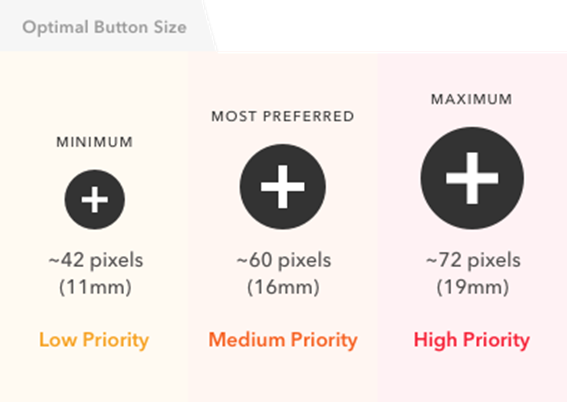
\includegraphics[width=0.5\linewidth]{figuras/optimal_button_size.png}
    \caption{Tamaño óptimo de botones según su prioridad}
    \label{fig:botones_optimos}
\end{figure}


Asimismo, la ubicación de los botones es fundamental para la usabilidad. Los usuarios están acostumbrados a interactuar con dispositivos digitales a lo largo del día y tienden a buscar ciertos elementos en ubicaciones predecibles. Por esta razón, es importante posicionar los botones en lugares donde los usuarios esperan encontrarlos, como en la parte inferior de la pantalla para acciones frecuentes o en la esquina superior derecha para opciones adicionales. Esta previsibilidad mejora la eficiencia y reduce la frustración del usuario \cite{Pickaso2022}.

\begin{figure} [h]
    \centering
    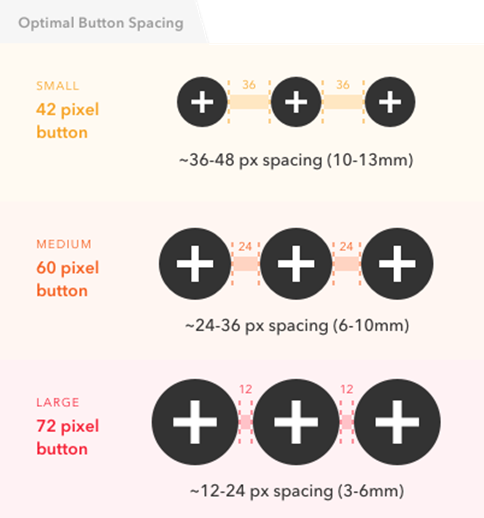
\includegraphics[width=0.5\linewidth]{figuras/optimal_space_buttons.png}
    \caption{Espaciado óptimo de botones según su tamaño}
    \label{fig:esapcio_optimo}
\end{figure}


\subsubsection{Diseño Responsivo}
El diseño responsivo es crucial para aplicaciones móviles, ya que asegura que la interfaz se adapte a diferentes tamaños de pantalla y resoluciones \cite{Becos2024}.

Dado que las pantallas de los dispositivos móviles varían en densidad, con más píxeles por pulgada en pantallas de mayor resolución, es importante utilizar píxeles independientes de la densidad (dp) para definir las dimensiones de los elementos de la interfaz. Esto asegura que los elementos mantengan su tamaño y proporción adecuados en diferentes dispositivos, proporcionando uniformidad y coherencia visual \cite{Pickaso2022}.

\subsubsection{Principios de Diseño}
Hay una serie de principios de diseño de interfaces para lograr que el producto digital satisfaga al cliente final \cite{AnonimoUX}.

\begin{itemize}
    \item \textbf{Simplicidad}: Es crucial evitar elementos innecesarios que puedan causar confusión \cite{AnonimoUX}.
    \item \textbf{Consistencia}: Al emplear elementos comunes en la interfaz de usuario, los usuarios se sienten más cómodos y familiarizados con el diseño, lo que facilita el uso del producto digital \cite{AnonimoUX}.
    \item \textbf{Jerarquía y manejo de espacios}: La disposición y estructuración de los elementos según su importancia ayuda a dirigir la atención del usuario a la información más relevante. Agrupar elementos relacionados crea una relación visual y mejora la comprensión del contenido \cite{AnonimoUX}.
    \item \textbf{Color y tipografía}: El color es esencial en el diseño de interfaces. Ajustar la saturación, luz y contraste del color en el diseño destaca elementos importantes y facilita la navegación. Asimismo, se utilizan diferentes tamaños, fuentes y disposiciones del texto para mejorar la legibilidad y jerarquía visual \cite{AnonimoUX}.
\end{itemize}

\subsubsection{Paleta de Colores}
Los colores desempeñan un papel fundamental en el diseño de interfaces de usuario, ya que no solo aportan personalidad y estilo al producto digital, sino que también influyen en la percepción y emociones del usuario \cite{EspacioUXSF}.

Una paleta de colores bien diseñada ayuda a los usuarios a comprender rápidamente la importancia y la relación entre diferentes elementos en la interfaz, como las llamadas a la acción o la información crítica. Al asignar colores específicos a distintas categorías o secciones, los usuarios pueden identificar fácilmente su ubicación en la interfaz y cómo navegar dentro de ella \cite{EspacioUXSF}.

La paleta de colores se elige para evocar emociones específicas que se alineen con los objetivos del diseño. Por ejemplo, los colores cálidos como el rojo y el naranja pueden provocar sensaciones de urgencia o excitación, lo que los hace ideales para botones de compra o alertas. En contraste, los colores fríos como el azul y el verde pueden inducir sensaciones de tranquilidad y confianza, siendo perfectos para páginas de inicio o secciones de información \cite{EspacioUXSF}.

Es esencial que la paleta de colores tenga en cuenta la legibilidad y la visibilidad, cumpliendo con los estándares de contraste y asegurando que la información sea clara para todos los usuarios \cite{EspacioUXSF}.

\subsubsection{Selección de Tipografía}
Al igual que la paleta de colores, la elección de una tipografía tiene un impacto significativo en el diseño de un producto digital. La tipografía moldea la manera en que se percibe y comprende la información visual. Elementos tipográficos como el tipo de letra, su tamaño y color tienen la capacidad de transmitir diversos significados y causar distintas respuestas emocionales \cite{CamaraSevilla2023}.

Una tipografía bien elegida mejora y facilita la comprensión y asimilación de la información por parte de los usuarios. Por ejemplo, una fuente en negrita y con letras mayúsculas puede transmitir fuerza y determinación, mientras que una tipografía delicada y manuscrita puede evocar elegancia y sofisticación. En contraste, una tipografía inadecuada puede dificultar la lectura, causar fatiga visual e incluso generar confusión o frustración en el usuario \cite{CamaraSevilla2023}.

Las tipografías se pueden clasificar según sus características:

\begin{itemize}
    \item \textbf{Fuentes Serif}: Estas fuentes se caracterizan por tener pequeños remates en los extremos de las letras, transmitiendo una sensación de formalidad. Ejemplos populares incluyen Times New Roman y Georgia \cite{CamaraSevilla2023}.
    \item \textbf{Fuentes Sans Serif}: Carecen de remates, lo que les confiere una apariencia más moderna y limpia. Se utilizan comúnmente en proyectos digitales. Ejemplos comunes son Arial, Helvetica y Calibri \cite{CamaraSevilla2023}.
    \item \textbf{Fuentes Script o Manuscritas}: Estas fuentes imitan la escritura a mano y suelen transmitir una sensación de personalización y creatividad. Ejemplos incluyen Brush Script y Pacifico \cite{CamaraSevilla2023}.
    \item \textbf{Fuentes Decorativas}: Son variadas y altamente estilizadas, utilizadas con fines ornamentales y para llamar la atención. Pueden ser temáticas o artísticas, como las fuentes de Navidad o títulos de películas \cite{CamaraSevilla2023}.
    \item \textbf{Fuentes Monoespaciadas}: Cada carácter ocupa el mismo espacio horizontal, lo que es útil en programación y diseño de tablas. Ejemplos son Courier New y Consolas \cite{CamaraSevilla2023}.
    \item \textbf{Fuentes Display}: Estas fuentes son diseñadas para títulos y encabezados, siendo llamativas y de alto impacto visual. Ejemplos incluyen Impact y Lobster \cite{CamaraSevilla2023}.
    \item \textbf{Fuentes Dingbats}: Contienen símbolos y caracteres especiales en lugar de letras y números, útiles para la creación de iconos y elementos gráficos. Wingdings y Webdings son ejemplos conocidos \cite{CamaraSevilla2023}.
\end{itemize}

Seleccionar la tipografía correcta es esencial para asegurar que el mensaje se transmita de manera eficaz y atractiva para los productos digitales. Hay varios factores clave que se deben considerar para conseguirlo \cite{CamaraSevilla2023}:

\begin{itemize}
    \item \textbf{Legibilidad}: La tipografía debe ser fácil de leer para el público objetivo. Esto incluye considerar el tamaño de la fuente, el espaciado entre letras y palabras, y la claridad de las formas de las letras \cite{CamaraSevilla2023}.
    \item \textbf{Personalidad}: La tipografía debe reflejar la identidad y los valores del producto digital \cite{CamaraSevilla2023}.
    \item \textbf{Consistencia}: Mantener una apariencia uniforme a lo largo del diseño refuerza la identidad visual y facilita la navegación del usuario \cite{CamaraSevilla2023}.
    \item \textbf{Jerarquía}: Utilizar variaciones en la tipografía, como tamaños y estilos (negritas, cursivas), para establecer una jerarquía de información ayuda a los usuarios a identificar elementos clave como títulos, subtítulos y texto principal \cite{CamaraSevilla2023}.
    \item \textbf{Combinación de Fuentes}: Seleccionar dos o más fuentes que se complementen puede enriquecer el diseño \cite{CamaraSevilla2023}.
    \item \textbf{Tamaño y Espaciado}: El tamaño de la fuente y el espaciado entre líneas afectan la legibilidad y la estética \cite{CamaraSevilla2023}.
\end{itemize}

\section{Experiencia de Usuario (UX)}
\subsection{Definición de UX (Experiencia de Usuario)}
La experiencia de usuario (UX) se refiere a las percepciones, sentimientos y respuestas que los usuarios tienen al interactuar con un producto digital \cite{Chacon2024}.

\subsection{Diferencias entre UX y UI}
El diseño de interfaz de usuario (UI) y la experiencia de usuario (UX) son conceptos estrechamente relacionados, pero tienen enfoques distintos y desempeñan roles específicos en el desarrollo de productos digitales. Mientras que UX se enfoca en el recorrido y en las interacciones de un usuario en todo el producto digital, UI se centra en cómo se ve y funciona el producto \cite{Chacon2024}.

\subsection{Tipos de experiencia de usuario}
Existen diferentes tipos de experiencia que pueden influir en cómo un usuario percibe un producto digital:

\begin{itemize}
    \item \textbf{Experiencia de navegación}: Se refiere a la forma en que un usuario se desplaza por un producto digital. Incluye la estructura de la navegación y la lógica que conecta las diferentes secciones o páginas. Una navegación intuitiva permite a los usuarios encontrar rápidamente la información que buscan. Por ejemplo, un menú de navegación claro y bien organizado facilita el movimiento entre las distintas secciones de una aplicación \cite{Chacon2024}.
    \item \textbf{Experiencia de usabilidad}: Se enfoca en cómo los usuarios interactúan con los elementos del producto digital. La usabilidad asegura que todos los componentes, como botones, barras de desplazamiento y formularios, funcionen correctamente y de manera consistente. Por ejemplo, un botón que responde rápidamente al ser presionado y realiza la acción esperada contribuye a una experiencia de usuario positiva \cite{Chacon2024}.
    \item \textbf{Experiencia Sensorial}: Involucra los elementos que impactan sensorialmente al usuario, como colores, disposición de elementos, sonidos y animaciones. Estos factores pueden influir significativamente en la percepción emocional del usuario respecto al producto. Por ejemplo, colores suaves y animaciones fluidas pueden crear una sensación de tranquilidad y profesionalismo, mientras que colores vibrantes y sonidos dinámicos pueden generar una sensación de energía y entusiasmo \cite{Chacon2024}.
\end{itemize}

\subsection{Proceso de experiencia de usuario}
La construcción de la experiencia de usuario para un producto se divide en varias etapas, cada una con su propio conjunto de actividades y herramientas \cite{Leon2013}:

\begin{itemize}
    \item \textbf{Investigación}: En esta etapa, se evalúan las necesidades de los clientes y se recopilan datos cruciales para entender mejor el contexto y las expectativas del usuario. Las técnicas más comunes incluyen \cite{Leon2013}:
    \begin{itemize}
        \item \textbf{Entrevistas:} Proveen información detallada directamente de los usuarios, ayudando a entender sus necesidades, deseos y problemas específicos \cite{Semi2022}.
        \item \textbf{Encuestas y Cuestionarios:} Recogen datos cuantitativos de una muestra más grande de usuarios, permitiendo identificar tendencias y patrones  \cite{Semi2022}.
        \item \textbf{Personas:} Creación de arquetipos basados en datos reales para representar diferentes tipos de usuarios  \cite{Semi2022}.
        \item \textbf{Mapas de Empatía:} Herramientas visuales que ayudan a comprender mejor a los usuarios, enfocándose en lo que piensan, sienten, dicen y hacen  \cite{Semi2022}.
        \item \textbf{Mapa de Experiencia del cliente:} Ilustra la experiencia completa de un usuario con un producto  \cite{Semi2022}.
        \item \textbf{Planteamiento del problema:} Define claramente los desafíos que el producto debe abordar  \cite{Semi2022}.
        \item \textbf{Diagramas de afinidad:} Organizan y agrupan información en categorías significativas  \cite{Semi2022}.
        \item \textbf{Análisis de la competencia:} Recopila información sobre tecnologías similares y reseñas de productos existentes  \cite{Semi2022}.
    \end{itemize}

\begin{figure}[h]
    \centering
    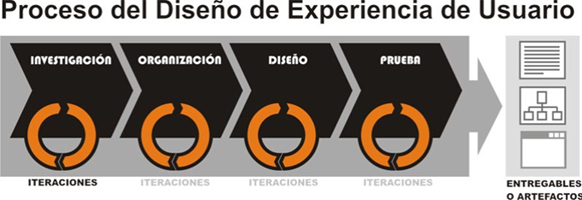
\includegraphics[width=0.5\linewidth]{figuras/proceso_diseno.png}
    \caption{Proceso de Diseño de Experencia de Usuario}
    \label{fig:enter-label}
\end{figure}

    
    \item \textbf{Organización}: Organiza toda la información obtenida durante la etapa de investigación utilizando herramientas como \cite{Leon2013}:
    \begin{itemize}
        \item \textbf{Mapa de Sitio:} Describe las páginas principales de un sitio y su relación, mostrando cómo se conectan  \cite{Semi2022}.
        \item \textbf{Flujo de Usuarios:} Diagrama que muestra la ruta que tomará un usuario en una aplicación para completar una tarea  \cite{Semi2022}.
        \item \textbf{Estructura Alámbrica/ Wireframes:} Visualización 2D de un producto digital, que va desde bocetos básicos a lápiz hasta diseños digitales interactivos (de baja, media y alta fidelidad)  \cite{Semi2022}.
    \end{itemize}
    \item \textbf{Diseño}: En la etapa de creación de prototipos, los wireframes de alta fidelidad se transforman en demostraciones interactivas que simulan fielmente la apariencia y el comportamiento del producto. Aquí se integra la investigación realizada en UI, considerando colores, tipografía, tamaños y espaciado de elementos, iconografía, entre otros. Las herramientas utilizadas incluyen Figma, Sketch y Adobe XD  \cite{Semi2022}.
    \item \textbf{Prueba}: Al finalizar la implementación, se realizan pruebas para asegurar que el producto cumple con las necesidades y expectativas de los usuarios  \cite{Semi2022}.
\end{itemize}

\section{Desarrollo Móvil en Android}
\subsection{Razones para elegir Android como plataforma de desarrollo}
Una de las razones principales para elegir Android como plataforma de desarrollo es su alta popularidad Guatemala. Según estudio la mayoría de celulares usados en el país son Samsung y Huawei, los cuales tienen sistema operativo Android \cite{Anonimo2019}.

Según datos recientes, Android domina el tráfico web móvil en el país, con un 82.50\% de participación. Esto significa que la mayoría de los usuarios de dispositivos móviles en Guatemala utilizan este sistema operativo, lo que amplía significativamente el alcance y la accesibilidad del producto desarrollado en esta plataforma \cite{Shum2023}.

\begin{figure} [h]
    \centering
    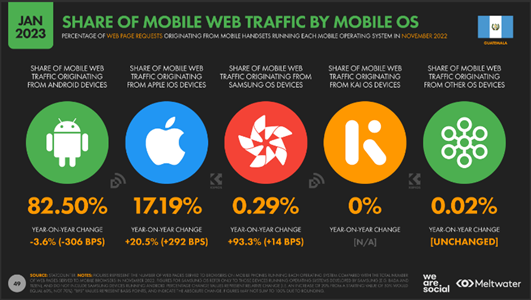
\includegraphics[width=0.5\linewidth]{figuras/mobile_web_traffic.png}
    \caption{Cuota de tráfico web móvil por sistema operativo}
    \label{fig:enter-label}
\end{figure}

Asimismo, Android es conocido por su diversidad en términos de dispositivos, desde teléfonos de alta gama hasta opciones más accesibles. También ofrece un alto nivel de flexibilidad y opciones de personalización, lo que facilita el desarrollo de aplicaciones. Finalmente, el ecosistema de desarrollo de Android está soportado con una vasta cantidad de recursos, herramientas y una comunidad activa de desarrolladores \cite{AnonimoAndroid}.

\subsection{Arquitectura de aplicaciones Android}
La arquitectura de una aplicación Android se basa en el patrón Modelo - Vista - Controlador (MVC). Aunque es muy común utilizar MVVM (Modelo - Vista - ViewModel), pues ofrece una separación más clara de la lógica de presentación y facilita el mantenimiento en comparación con MVC \cite{RamosSF}.

\subsubsection{Componentes}
\begin{itemize}
    \item \textbf{Modelo}: Contiene los datos, el estado y la lógica del negocio \cite{Bhadoria2013}.
    \item \textbf{Vista}: Representa la interfaz de usuario. Se comunica con el ViewModel a través de mecanismos de enlace de datos (data binding), permitiendo una actualización automática de la UI cuando cambian los datos \cite{Bhadoria2013}.
    \item \textbf{ViewModel}: Actúa como un intermediario entre el Modelo y la Vista. Expone datos y comandos que la Vista puede consumir y ejecutar, y notifica a la Vista sobre cambios en los datos utilizando observables (como LiveData) \cite{Bhadoria2013}.
\end{itemize}

\subsubsection{Flujo de Trabajo}
\begin{itemize}
    \item La Vista se enlaza automáticamente al ViewModel para observar los datos \cite{Bhadoria2013}.
    \item El ViewModel obtiene los datos del Modelo y prepara la lógica de presentación \cite{Bhadoria2013}.
    \item Cualquier cambio en el Modelo se refleja automáticamente en la Vista a través del ViewModel \cite{Bhadoria2013}.
    \item La interacción del usuario en la Vista invoca métodos en el ViewModel, que a su vez pueden actualizar el Modelo \cite{Bhadoria2013}.
\end{itemize}

\begin{figure}
    \centering
    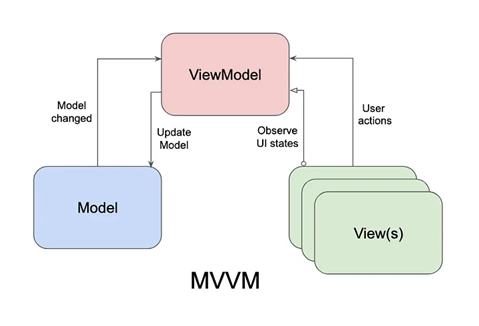
\includegraphics[width=0.5\linewidth]{figuras/mvvm.png}
    \caption{Diagrama de funcionamiento MVVM}
    \label{fig:enter-label}
\end{figure}

\subsection{Buenas prácticas de desarrollo Android}
Al desarrollar aplicaciones para Android, es esencial seguir ciertas buenas prácticas para asegurar la calidad y la eficiencia del producto final \cite{PhillipsStewart2022}:

\subsubsection{Uso de Layouts Adecuados}
\begin{itemize}
    \item \textbf{ConstraintLayout}: Es eficiente y flexible, permitiendo posicionar elementos de manera relativa a otros elementos \cite{PhillipsStewart2022}.
    \item \textbf{LinearLayout}: Organiza los elementos en una sola fila o columna, siendo útil para diseños sencillos y alineaciones básicas \cite{PhillipsStewart2022}.
    \item \textbf{RelativeLayout}: Permite posicionar los elementos en relación a otros elementos o a sus propios padres, ofreciendo más flexibilidad pero con un mayor costo de rendimiento comparado con ConstraintLayout \cite{PhillipsStewart2022}.
\end{itemize}

\subsubsection{Gestión de Recursos}
\begin{itemize}
    \item Utilizar unidades independientes de densidad (dp) para asegurar que los elementos de la interfaz mantengan su tamaño y proporciones adecuadas en dispositivos con diferentes tamaños de pantalla \cite{PhillipsStewart2022}.
    \item Definir colores, estilos y dimensiones en archivos de recursos para promover la reutilización y mantener la consistencia del diseño \cite{PhillipsStewart2022}.
    \item Utilizar Gradle para gestionar dependencias, lo que te permitirá mantener el código actualizado y seguro \cite{PhillipsStewart2022}.
\end{itemize}

\subsubsection{Optimización del Rendimiento}
\begin{itemize}
    \item Minimizar el uso de vistas anidadas para mejorar el rendimiento de la interfaz de usuario \cite{PhillipsStewart2022}.
    \item Evitar operaciones pesadas en el hilo principal \cite{PhillipsStewart2022}.
\end{itemize}

\subsubsection{Seguridad}
\begin{itemize}
    \item Proteger los datos del usuario mediante el uso de almacenamiento cifrado y permisos adecuados \cite{PhillipsStewart2022}.
    \item Validar las entradas del usuario para prevenir ataques de inyección y otras vulnerabilidades de seguridad \cite{PhillipsStewart2022}.
    \item Validar permisos de uso de almacenamiento, cámara, micrófono, etc para respetar las políticas de privacidad de Android \cite{PhillipsStewart2022}.
\end{itemize}

